\chapter{Camera calibration}

\begin{description}
    \item[World reference frame (WRF)] \marginnote{World reference frame (WRF)}
        Coordinate system $(X_W, Y_W, Z_W)$ of the real world relative to a reference point (e.g. a corner).

    \item[Camera reference frame (CRF)] \marginnote{Camera reference frame (CRF)}
        Coordinate system $(X_C, Y_C, Z_C)$ that characterizes a camera.

    \item[Image reference frame (IRF)] \marginnote{Image reference frame (IRF)}
        Coordinate system $(U, V)$ of the image.
        They are obtained as a perspective projection of CRF coordinates as:
        \[ 
            u = \frac{f}{z}x_C 
            \hspace{3em} 
            v = \frac{f}{z}y_C 
        \]

    \begin{figure}[H]
        \centering
        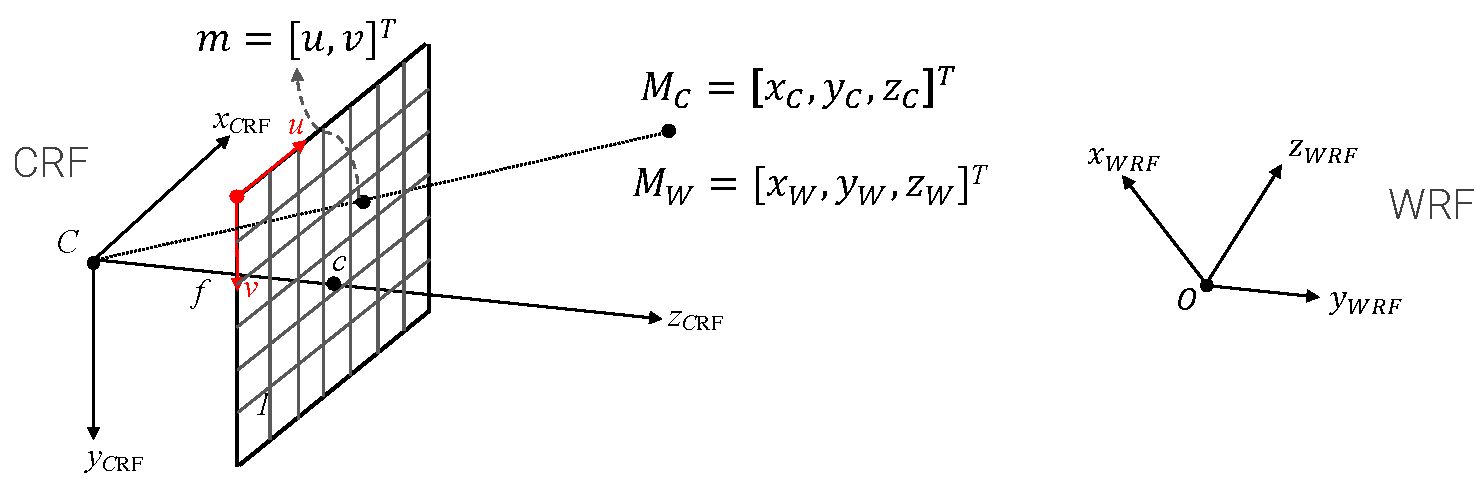
\includegraphics[width=0.8\linewidth]{./img/_formation_system.pdf}
        \caption{Example of WRF, CRF and IRF}
    \end{figure}
\end{description}



\section{Forward imaging model}


\subsection{Image pixelization (CRF to IRF)}
\marginnote{Image pixelization}

The conversion from the camera reference frame to the image reference frame
is done in two steps:
\begin{descriptionlist}
    \item[Discretization] \marginnote{Discretization}
        Given the sizes (in mm) $\Delta u$ and $\Delta v$ of the pixels,
        it is sufficient to modify the perspective projection to map CRF coordinates into a discrete grid:
        \[ 
            u = \frac{1}{\Delta u}\frac{f}{z_C}x_C 
            \hspace{3em} 
            v = \frac{1}{\Delta v}\frac{f}{z_C}y_C 
        \]

    \item[Origin translation] \marginnote{Origin translation}
        To avoid negative pixels, the origin of the image has to be translated from the piercing point $c$ to the top-left corner.
        This is done by adding an offset $(u_0, v_0)$ to the projection (in the new system, $c = (u_0, v_0)$):
        \[ 
            u = \frac{1}{\Delta u}\frac{f}{z_C}x_C + u_0
            \hspace{3em} 
            v = \frac{1}{\Delta v}\frac{f}{z_C}y_C +v_0
        \]

    \begin{figure}[H]
        \centering
        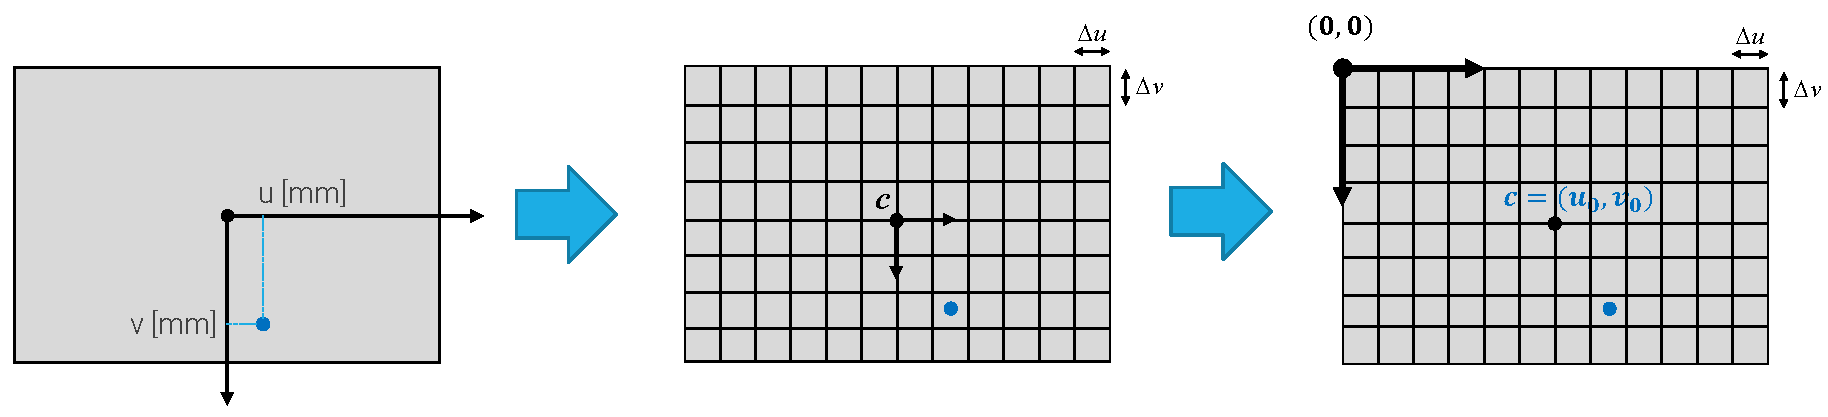
\includegraphics[width=0.9\linewidth]{./img/_pixelization.pdf}
        \caption{Pixelization process}
    \end{figure}

    \item[Intrinsic parameters] \marginnote{Intrinsic parameters}
        By fixing $f_u = \frac{f}{\Delta u}$ and $f_v = \frac{f}{\Delta v}$, the projection can be rewritten as:
        \[ 
            u = f_u\frac{x_C}{z_C} + u_0
            \hspace{3em} 
            v = f_v\frac{y_C}{z_C} +v_0
        \]
        Therefore, there is a total of 4 parameters: $f_u$, $f_v$, $u_0$ and $v_0$.
        
        \begin{remark}
            A more general model includes a further parameter (skew)
            to account for non-orthogonality between the axes of the image sensor such as:
            \begin{itemize}
                \item Misplacement of the sensor so that it is not perpendicular to the optical axis.
                \item Manufacturing issues.
            \end{itemize}

            Nevertheless, in practice skew is always 0.
        \end{remark}
\end{descriptionlist}


\subsection{Roto-translation (WRF to CRF)}
\marginnote{Roto-translation}

The conversion from the world reference system to the camera reference system
is done through a roto-translation w.r.t. the optical center.

Given: 
\begin{itemize}
    \item A WRF point $\vec{M}_W = (x_W, y_W, z_W)$,
    \item A rotation matrix $\matr{R}$,
    \item A translation vector $\vec{t}$,
\end{itemize}
the coordinates $\vec{M}_C$ in CRF corresponding to $\vec{M}_W$ are given by:
\[  
    \vec{M}_C = \begin{bmatrix} x_C \\ y_C \\ z_C \end{bmatrix} =
    \matr{R}\vec{M}_W + \vec{t} =
    \begin{bmatrix}
        r_{1,1} & r_{1,2} & r_{1,3} \\
        r_{2,1} & r_{2,2} & r_{2,3} \\
        r_{3,1} & r_{3,2} & r_{3,3} \\
    \end{bmatrix}
    \begin{bmatrix}
        x_W \\ y_W \\ z_W
    \end{bmatrix}
    +
    \begin{bmatrix}
        t_1 \\ t_2 \\ t_3
    \end{bmatrix}
\]

\begin{remark}
    The coordinates $\vec{C}_W$ of the optical center $\vec{C} = \nullvec$ are obtained as:
    \[ 
        \nullvec = \matr{R}\vec{C}_W + \vec{t} 
            \iff (\nullvec - \vec{t}) = \matr{R}\vec{C}_W 
            \iff \vec{C}_W = \matr{R}^T (\nullvec - \vec{t})
            \iff \vec{C}_W = -\matr{R}^T\vec{t}
    \]
\end{remark}

\begin{description}
    \item[Extrinsic parameters] \marginnote{Extrinsic parameters}
        \phantom{}
        \begin{itemize}
            \item The rotation matrix $\matr{R}$ has 9 elements of which 3 are independent (i.e. the rotation angles around the axes). 
            \item The translation matrix $\vec{t}$ has 3 elements.
        \end{itemize}

        Therefore, there is a total of 6 parameters.
\end{description}


\begin{remark}
    It is not possible to combine the intrinsic camera model and the extrinsic roto-translation to
    create a linear model for the forward imaging model.
    \[
        u = f_u \frac{r_{1,1}x_W + r_{1,2}y_W + r_{1,3}z_W + t_1}{r_{3,1}x_W + r_{3,2}y_W + r_{3,3}z_W + t_3} + u_0
        \hspace{1.5em}
        v = f_v \frac{r_{2,1}x_W + r_{2,2}y_W + r_{2,3}z_W + t_2}{r_{3,1}x_W + r_{3,2}y_W + r_{3,3}z_W + t_3} + v_0
    \]
\end{remark}



\section{Projective space}

\begin{remark}
    In the 2D Euclidean plane $\mathbb{R}^2$, parallel lines never intersect and points at infinity cannot be represented.
    \begin{figure}[H]
        \centering
        \begin{subfigure}{0.45\linewidth}
            \centering
            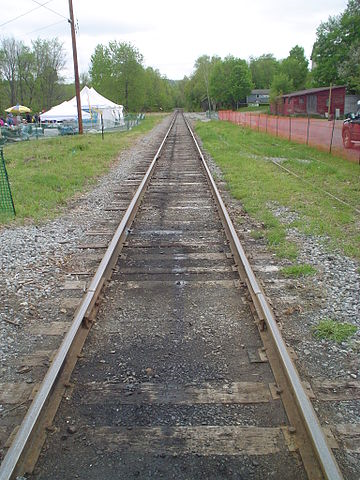
\includegraphics[width=0.45\linewidth]{./img/point_infinity_example1.png}
        \end{subfigure}
        \begin{subfigure}{0.45\linewidth}
            \centering
            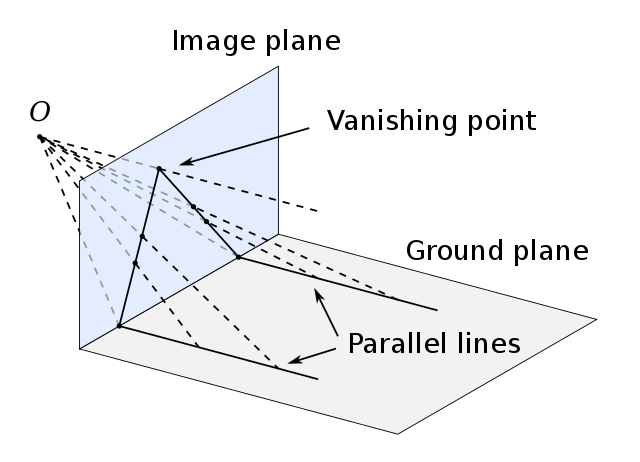
\includegraphics[width=0.8\linewidth]{./img/point_infinity_example2.png}
        \end{subfigure}
        \caption{Example of point at infinity}
    \end{figure}
\end{remark}

\begin{remark}
    Point at infinity is a point in space while the vanishing point is in the image plane.
\end{remark}

\begin{description}
    \item[Homogeneous coordinates] \marginnote{Homogeneous coordinates}
        Without loss of generality, consider the 2D Euclidean space $\mathbb{R}^2$.

        Given a coordinate $(u, v)$ in Euclidean space, its homogeneous coordinates have an additional dimension
        such that:
        \[ (u, v) \equiv (ku, kv, k) \,\forall k \neq 0 \]
        In other words, a 2D Euclidean point is represented by an equivalence class of 3D points.

    \item[Projective space] \marginnote{Projective space}
        Space $\mathbb{P}^n$ associated with the homogeneous coordinates of an Euclidean space $\mathbb{R}^n$.

        \begin{figure}[H]
            \centering
            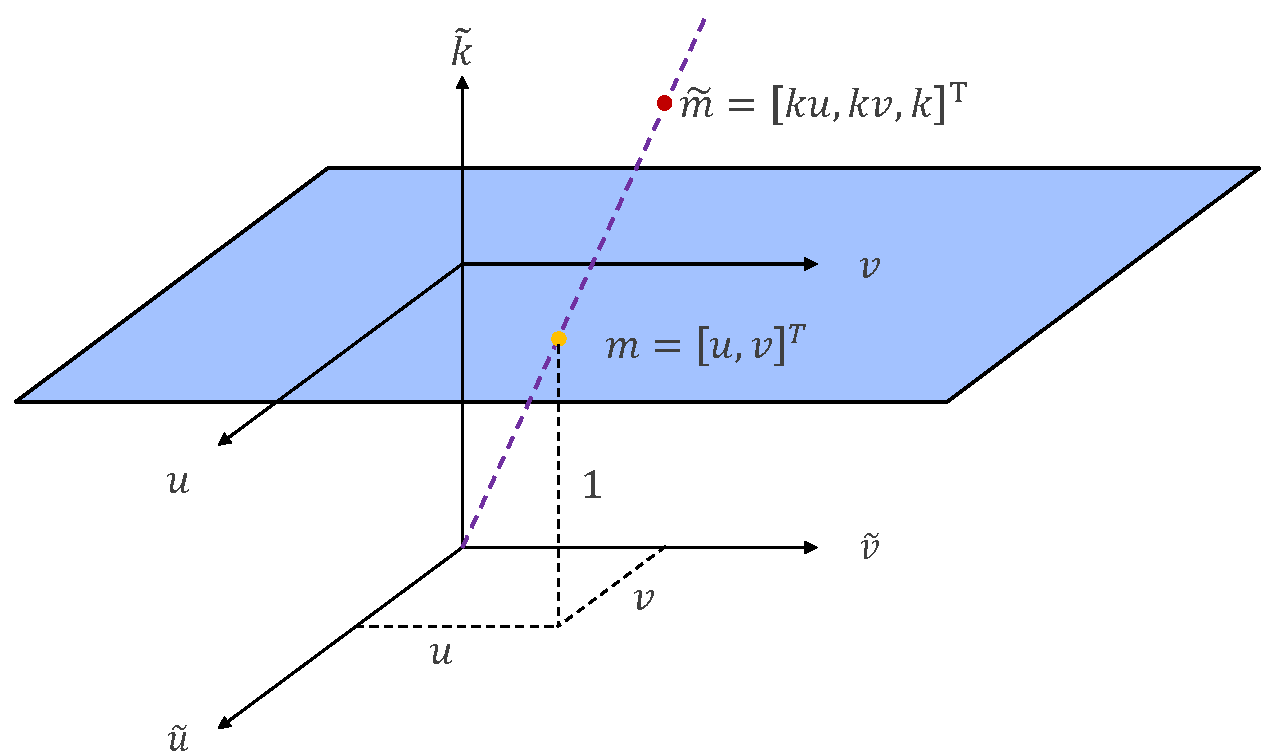
\includegraphics[width=0.6\linewidth]{./img/_projective_space.pdf}
            \caption{Example of projective space $\mathbb{P}^2$}
        \end{figure}

        \begin{remark}
            $\nullvec$ is not a valid point in $\mathbb{P}^n$.
        \end{remark}

        \begin{remark}
            A projective space allows to homogeneously handle both ordinary (image) and ideal (scene) points without introducing additional complexity.
        \end{remark}

    \item[Point at infinity] \marginnote{Point at infinity}
        Given the parametric equation of a 2D line defined as:
        \[ 
            \vec{m} = \vec{m}_0 + \lambda \vec{d} = 
            \begin{bmatrix} u_0 \\ v_0 \end{bmatrix} + \lambda \begin{bmatrix} a \\ b \end{bmatrix} =
            \begin{bmatrix} u_0 + \lambda a \\ v_0 + \lambda b \end{bmatrix}
        \]
        It is possible to define a generic point in the projective space along the line $m$ as:
        \[ 
            \tilde{\vec{m}} \equiv 
            \begin{bmatrix} \vec{m} \\ 1 \end{bmatrix} \equiv
            \begin{bmatrix} u_0 + \lambda a \\ v_0 + \lambda b \\ 1 \end{bmatrix} \equiv
            \begin{bmatrix} \frac{u_0}{\lambda} + a \\ \frac{v_0}{\lambda} + b \\ \frac{1}{\lambda} \end{bmatrix}
        \]

        The projective coordinates $\tilde{\vec{m}}_\infty$ of the point at infinity of a line $m$ is given by:
        \[ \tilde{\vec{m}}_\infty = \lim_{\lambda \rightarrow \infty} \tilde{\vec{m}} \equiv \begin{bmatrix} a \\ b \\ 0 \end{bmatrix} \]

        \begin{figure}[H]
            \centering
            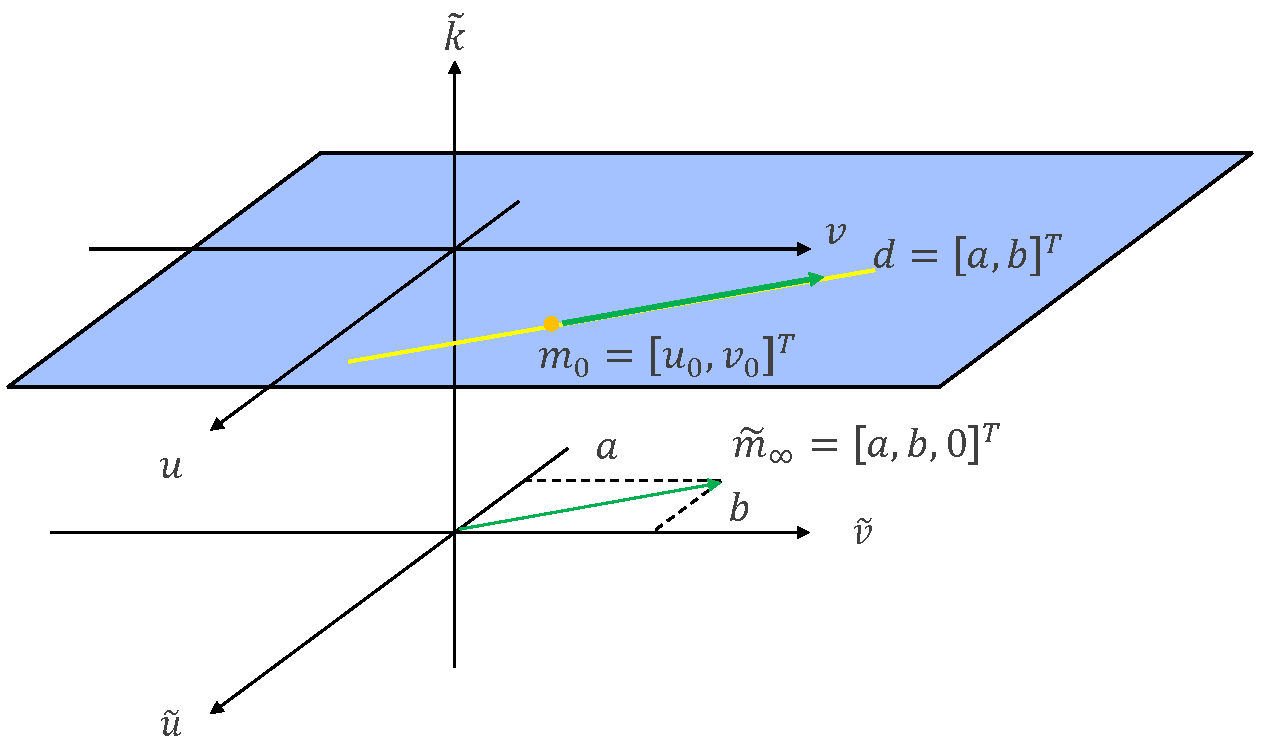
\includegraphics[width=0.6\linewidth]{./img/_projective_point_inifinity.pdf}
            \caption{Example of infinity point in $\mathbb{P}^2$}
        \end{figure}

        In 3D, the definition is trivially extended as:
        \[ 
            \tilde{\vec{M}}_\infty = 
            \lim_{\lambda \rightarrow \infty} \begin{bmatrix} \frac{x_0}{\lambda} + a \\ \frac{y_0}{\lambda} + b \\ \frac{z_0}{\lambda} + c \\ \frac{1}{\lambda} \end{bmatrix} \equiv
            \begin{bmatrix} a \\ b \\ c \\ 0 \end{bmatrix}
        \]

    \item[Perspective projection] \marginnote{Perspective projection in projective space}
        Given a point $\vec{M}_C = (x_C, y_C, z_C)$ in the CRF and its corresponding point $\vec{m} = (u, v)$ in the image,
        the non-linear perspective projection in Euclidean space can be done linearly in the projective space as:
        \[  
            \begin{split}
                \tilde{\vec{m}} &\equiv 
                \begin{bmatrix} u \\ v \\ 1 \end{bmatrix} \equiv
                \begin{bmatrix} f_u\frac{x_C}{z_C} + u_0 \\ f_v\frac{y_C}{z_C} +v_0 \\ 1 \end{bmatrix} \equiv
                z_C \begin{bmatrix} f_u\frac{x_C}{z_C} + u_0 \\ f_v\frac{y_C}{z_C} +v_0 \\ 1 \end{bmatrix} \\
                &\equiv \begin{bmatrix} f_u x_C + z_C u_0 \\ f_v y_C + z_C v_0 \\ z_C \end{bmatrix} \equiv
                \begin{bmatrix} f_u & 0 & u_0 & 0 \\ 0 & f_v & v_0 & 0 \\ 0 & 0 & 1 & 0 \end{bmatrix} \begin{bmatrix} x_C \\ y_C \\ z_C \\ 1 \end{bmatrix} \equiv
                \matr{P}_\text{int} \tilde{\vec{M}}_C
            \end{split}
        \]

        \begin{remark}
            The equation can be written to take account of the arbitrary scale factor $k$ as:
            \[ k\tilde{\vec{m}} = \matr{P}_\text{int} \tilde{\vec{M}}_C \]
            or, if $k$ is omitted, as:
            \[ \tilde{\vec{m}} \approx \matr{P}_\text{int} \tilde{\vec{M}}_C \]
        \end{remark}

        \begin{remark}
            In projective space, we can also project in Euclidean space the point at infinity of parallel 3D lines in CRF with direction $(a, b, c)$:
            \[ 
                \tilde{\vec{m}}_\infty \equiv 
                    \matr{P}_\text{int} \begin{bmatrix} a \\ b \\ c \\ 0 \end{bmatrix} \equiv
                    \begin{bmatrix} f_u & 0 & u_0 & 0 \\ 0 & f_v & v_0 & 0 \\ 0 & 0 & 1 & 0 \end{bmatrix} \begin{bmatrix} a \\ b \\ c \\ 0 \end{bmatrix} \equiv
                    \begin{bmatrix} f_u a + c u_0 \\ f_v b + c v_0 \\ c \end{bmatrix} \equiv
                    c\begin{bmatrix} f_u \frac{a}{c} + u_0 \\ f_v \frac{b}{c} + v_0 \\ 1 \end{bmatrix}
            \]
            Therefore, the Euclidean coordinates are:
            \[ \vec{m}_\infty = \begin{bmatrix} f_u \frac{a}{c} + u_0 \\ f_v \frac{b}{c} + v_0 \end{bmatrix} \]
            
            Note that this is not possible when $c = 0$ (i.e. the line is parallel to the image plane).
        \end{remark}

    \item[Intrinsic parameter matrix] \marginnote{Intrinsic parameter matrix}
        The intrinsic transformation can be expressed through a matrix:
        \[ 
            \matr{A} = 
                \begin{bmatrix}
                    f_u & 0 & u_0 \\ 0 & f_v & v_0 \\ 0 & 0 & 1
                \end{bmatrix} 
        \]
        $\matr{A}$ is always upper right triangular and models the characteristics of the imaging device.
        
        \begin{remark}
            If skew is considered, it would be at position $(1, 2)$.
        \end{remark}

    \item[Extrinsic parameter matrix] \marginnote{Extrinsic parameter matrix}
        The extrinsic transformation can be expressed through a matrix:
        \[ 
            \matr{G} =  
            \begin{bmatrix} \matr{R} & \vec{t} \\ \nullvec & 1 \end{bmatrix} =
            \begin{bmatrix} 
                r_{1,1} & r_{1,2} & r_{1,3} & t_1 \\ 
                r_{2,1} & r_{2,2} & r_{2,3} & t_2 \\ 
                r_{3,1} & r_{3,2} & r_{3,3} & t_3 \\ 
                0 & 0 & 0 & 1
            \end{bmatrix}
        \]

    \item[Perspective projection matrix (PPM)] \marginnote{Perspective projection matrix}
        As the following hold: 
        \[
            \matr{P}_\text{int} = [ \matr{A} | \nullvec ] \hspace{3em} \tilde{\vec{M}}_C \equiv \matr{G} \tilde{\vec{M}}_W
        \]
        The perspective projection can be represented in matrix form as:
        \[ \tilde{\vec{m}} \equiv \matr{P}_\text{int} \tilde{\vec{M}}_C \equiv \matr{P}_\text{int} \matr{G} \tilde{\vec{M}}_W \equiv \matr{P} \tilde{\vec{M}}_W \]
        where $\matr{P} = \matr{P}_\text{int} \matr{G}$ is the perspective projection matrix. It is full-rank and has shape $3 \times 4$.

        \begin{remark}
            Every full-rank $3 \times 4$ matrix is a PPM.
        \end{remark}

        \begin{description}
            \item[Canonical perspective projection] \marginnote{Canonical perspective projection}
                PPM of form:
                \[ \matr{P} \equiv [\matr{I} | \nullvec] \]

                It is useful to represent the core operations carried out by a perspective projection as any general PPM can be factorized as:
                \[ \matr{P} \equiv \matr{A} [\matr{I} | \nullvec] \matr{G} \]
                where:
                \begin{itemize}
                    \item $\matr{G}$ converts from WRT to CRF.
                    \item $[\matr{I} | \nullvec]$ performs the canonical perspective projection (i.e. divide by the third coordinate).
                    \item $\matr{A}$ applies camera specific transformations.
                \end{itemize}

                A further factorization is:
                \[ 
                    \matr{P} \equiv \matr{A} [\matr{I} | \nullvec] \matr{G} \equiv 
                    \matr{A}[\matr{I} | \nullvec] \begin{bmatrix} \matr{R} & \vec{t} \\ \nullvec & 1 \end{bmatrix} \equiv
                    \matr{A} [ \matr{R} | \vec{t} ]
                \]
        \end{description}
\end{description}



\section{Lens distortion}

The PPM is based on the pinhole model and is unable to capture distortions that a lens introduces.

\begin{description}
    \item[Radial distortion] \marginnote{Radial distortion}
        Deviation from the ideal pinhole caused by the lens curvature.

        \begin{descriptionlist}
            \item[Barrel distortion] \marginnote{Barrel distortion}
                Defect associated with wide-angle lenses that causes straight lines to bend outwards.
            \item[Pincushion distortion] \marginnote{Pincushion distortion}
                Defect associated with telephoto lenses that causes straight lines to bend inwards.
        \end{descriptionlist}

        \begin{figure}[H]
            \centering
            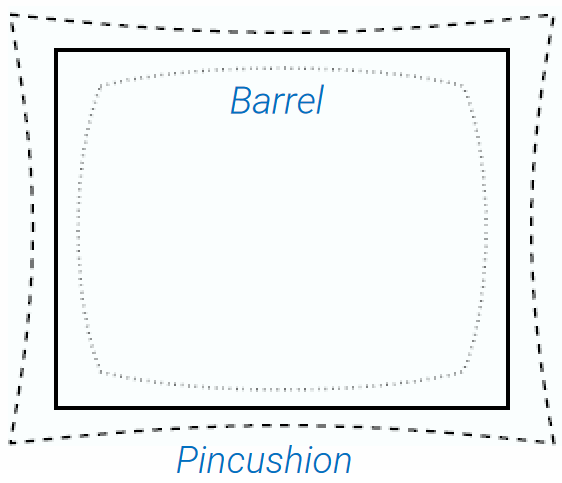
\includegraphics[width=0.25\linewidth]{./img/radial_distortion.png}
            \caption{Example of distortions w.r.t. a perfect rectangle}
        \end{figure}

    \item[Tangential distortion]
        Second-order effects caused by misalignment or defects of the lens (i.e. capture distortions that are not considered in radial distortion).
\end{description}


\subsection{Modeling lens distortion}
\marginnote{Modeling lens distortion}

Lens distortion can be modeled using a non-linear transformation that maps ideal (undistorted) image coordinates $(x_\text{undist}, y_\text{undist})$ into
the observed (distorted) coordinates $(x, y)$:
\[ 
    \begin{bmatrix} x \\ y \end{bmatrix} =
    \underbrace{ L(r) \begin{bmatrix} x_\text{undist} \\ y_\text{undist} \end{bmatrix} }_{\text{Radial distortion}} +
    \underbrace{ \begin{bmatrix} dx(x_\text{undist}, y_\text{undist}, r) \\ dy(x_\text{undist}, y_\text{undist}, r) \end{bmatrix} }_{\text{Tangential distortion}}
\]
where:
\begin{itemize}
    \item $r$ is the distance from the distortion center which is usually assumed to be the piercing point $c = (0, 0)$.
        Therefore, $r = \sqrt{ (x_\text{undist})^2 + (y_\text{undist})^2 }$.
    \item $L(r)$ is the radial distortion function which is a linear operator defined for positive $r$ only and is approximated using the Taylor series:
        \[ L(0) = 1 \hspace{2em} L(r) = 1 + k_1 r^2 + k_2 r^4 + k_3 r^6 + \dots \]
        where $k_i$ are additional intrinsic parameters.
    \item The tangential distortion is approximated as:
        \[ 
            \begin{bmatrix} dx(x_\text{undist}, y_\text{undist}, r) \\ dy(x_\text{undist}, y_\text{undist}, r) \end{bmatrix} =
            \begin{bmatrix} 
                2 p_1 x_\text{undist} y_\text{undist} + p_2 (r^2 + 2(x_\text{undist})^2) \\
                2 p_1 y_\text{undist} x_\text{undist} + p_2 (r^2 + 2(y_\text{undist})^2) \\
            \end{bmatrix}
        \]
        where $p_1$ and $p_2$ are additional intrinsic parameters.
        \begin{remark}
            This approximation has been empirically shown to work.
        \end{remark}
\end{itemize}

\begin{remark}
    The additivity of the two distortions in an assumption.
    Other models might add arbitrary complexity.
\end{remark}


\subsection{Image formation with lens distortion}
\marginnote{Image formation with lens distortion}

Lens distortion is applied after the canonical perspective projection.
Therefore, the complete workflow for image formation becomes the following:
\begin{enumerate}
    \item Transform points from WRF to CRF:
        \[ \matr{G} \tilde{\vec{M}}_W \equiv \begin{bmatrix} x_C & y_C & z_C & 1 \end{bmatrix}^T \]
    \item Apply the canonical perspective projection:
        \[ 
            \begin{bmatrix} \frac{x_C}{z_C} & \frac{y_C}{z_C} \end{bmatrix}^T =
            \begin{bmatrix} x_\text{undist} & y_\text{undist} \end{bmatrix}^T
        \]
    \item Apply the lens distortion non-linear mapping:
        \[ 
            L(r) \begin{bmatrix} x_\text{undist} \\ y_\text{undist} \end{bmatrix} +
            \begin{bmatrix} dx(x_\text{undist}, y_\text{undist}, r) \\ dy(x_\text{undist}, y_\text{undist}, r) \end{bmatrix} =
            \begin{bmatrix} x \\ y \end{bmatrix}
        \]
    \item Transform points from CRF to IRF:
        \[
            \matr{A} \begin{bmatrix} x \\ y \\ 1 \end{bmatrix} \equiv
            \begin{bmatrix} ku \\ kv \\ k \end{bmatrix} \mapsto
            \begin{bmatrix} u \\ v \end{bmatrix}
        \]
\end{enumerate}



\section{Zhang's method}

\begin{description}
    \item[Calibration patterns] \marginnote{Calibration patterns}
        There are two approaches to camera calibration:
        \begin{itemize}
            \item Use a single image of a 3D calibration object (i.e. image with at least 2 planes with a known pattern).
            \item Use multiple (at least 3) images of the same planar pattern (e.g. a chessboard).
        \end{itemize}

        \begin{remark}
            In practice, it is easier to get multiple images of the same pattern.
        \end{remark}

    \item[Algebraic error] \marginnote{Algebraic error}
        Error minimized to estimate an initial guess for a subsequent refinement step.
        It should be cheap to compute.
    
    \item[Geometric error] \marginnote{Geometric error}
        Error minimized to match the actual geometrical location of a problem.

    \item[Zhang's method] \marginnote{Zhang's method}
        Algorithm to determine the intrinsic and extrinsic parameters of a camera setup given multiple images of a pattern.

        \begin{description}
            \item[Image acquisition] 
                Acquire $n$ images of a planar pattern with $c$ internal corners.

                Consider a chessboard for which we have prior knowledge of:
                \begin{itemize}
                    \item The number of internal corners,
                    \item The size of the squares.
                \end{itemize}

                \begin{remark}
                    To avoid ambiguity, the number of internal corners should be odd along one axis and even along the other
                    (otherwise, a $180^\circ$ rotation of the board would be indistinguishable).
                \end{remark}

                The WRF can be defined such that:
                \begin{itemize}
                    \item The origin is always at the same corner of the chessboard.
                    \item The $z$-axis is at the same level of the pattern so that $z=0$ when referring to points of the chessboard.
                    \item The $x$ and $y$ axes are aligned to the grid of the chessboard. $x$ is aligned along the short axis and $y$ to the long axis.
                \end{itemize}

                \begin{remark}
                    As each image has its own extrinsic parameters,
                    during the execution of the algorithm, for each image $i$ will be computed
                    an estimate of its own extrinsic parameters $\matr{R}_i$ and $\vec{t}_i$.
                \end{remark}

                \begin{figure}[H]
                    \centering
                    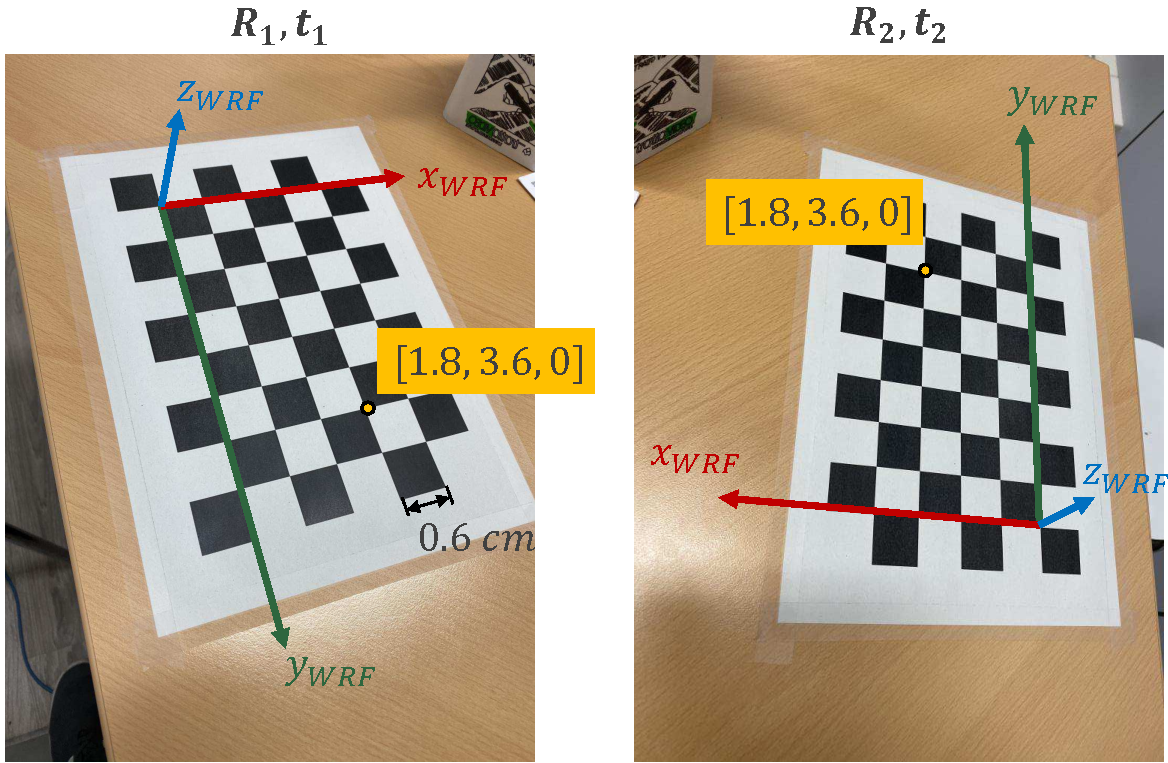
\includegraphics[width=0.4\linewidth]{./img/_zhang_image_acquistion.pdf}
                    \caption{Example of two acquired images}
                \end{figure}
        \end{description}

    \item[Initial homographies guess]
        For each image $i$, compute an initial guess of its homography $\matr{H}_i$.
        Due to the choice of the $z$-axis position, the perspective projection matrix and the WRF points can be simplified:
        \[ 
            \begin{split}
                k \tilde{\vec{m}} &= 
                k \begin{bmatrix} u \\ v \\ 1 \end{bmatrix} =
                \matr{P} \tilde{\vec{M}}_W =
                \begin{bmatrix}
                    p_{1,1} & p_{1,2} & \cancel{p_{1,3}} & p_{1,4} \\
                    p_{2,1} & p_{2,2} & \cancel{p_{2,3}} & p_{2,4} \\
                    p_{3,1} & p_{3,2} & \cancel{p_{3,3}} & p_{3,4}
                \end{bmatrix}
                \begin{bmatrix} x \\ y \\ \cancel{0} \\ 1 \end{bmatrix} \\
                &= \begin{bmatrix}
                    p_{1,1} & p_{1,2} & p_{1,4} \\
                    p_{2,1} & p_{2,2} & p_{2,4} \\
                    p_{3,1} & p_{3,2} & p_{3,4}
                \end{bmatrix}
                \begin{bmatrix} x \\ y \\ 1 \end{bmatrix} =
                \matr{H}\tilde{\vec{w}}
            \end{split}
        \]
        where $\matr{H}$ is a homography and represents a general transformation between projective planes.

        \begin{description}
            \item[DLT algorithm]
                Consider the $i$-th image with its $c$ corners.
                For each corner $j$, we have prior knowledge of:
                \begin{itemize}
                    \item Its 3D coordinates in the WRF.
                    \item Its 2D coordinates in the IRF.
                \end{itemize}
                Then, for each corner $j$, we can define 3 linear equations where the homography $\matr{H}_i$ of the $i$-th image is the unknown:
                \[ 
                    \tilde{\vec{m}}_{i,j} \equiv 
                        \begin{bmatrix} u_{i,j} \\ v_{i,j} \\ 1 \end{bmatrix} \equiv
                        \begin{bmatrix}
                            p_{i,1,1} & p_{i,1,2} & p_{i,1,4} \\
                            p_{i,2,1} & p_{i,2,2} & p_{i,2,4} \\
                            p_{i,3,1} & p_{i,3,2} & p_{i,3,4} \\
                        \end{bmatrix}
                        \begin{bmatrix} x_j \\ y_j \\ 1 \end{bmatrix} \equiv
                        \matr{H}_i \tilde{\vec{w}}_j \equiv
                        \underset{\mathbb{R}^{3 \times 3}}{\begin{bmatrix}
                            \vec{h}_{i, 1}^T \\ \vec{h}_{i, 2}^T \\ \vec{h}_{i, 3}^T
                        \end{bmatrix}}
                        \tilde{\vec{w}}_j \equiv
                        \underset{\mathbb{R}^{3 \times 1}}{\begin{bmatrix}
                            \vec{h}_{i, 1}^T \tilde{\vec{w}}_j \\ 
                            \vec{h}_{i, 2}^T \tilde{\vec{w}}_j \\ 
                            \vec{h}_{i, 3}^T \tilde{\vec{w}}_j
                        \end{bmatrix}}
                \]
                Geometrically, we can interpret $\matr{H}_i \tilde{\vec{w}}_j$ as a point in $\mathbb{P}^2$
                that we want to align to the projection of $(u_{i,j}, v_{i,j})$ by tweaking $\matr{H}_i$
                (i.e. find $\matr{H}_i^*$ such that $\matr{H}_i^* \tilde{\vec{w}}_j \equiv k \begin{bmatrix} u_{i,j} & v_{i,j} & 1 \end{bmatrix}^T$).
                \begin{center}
                    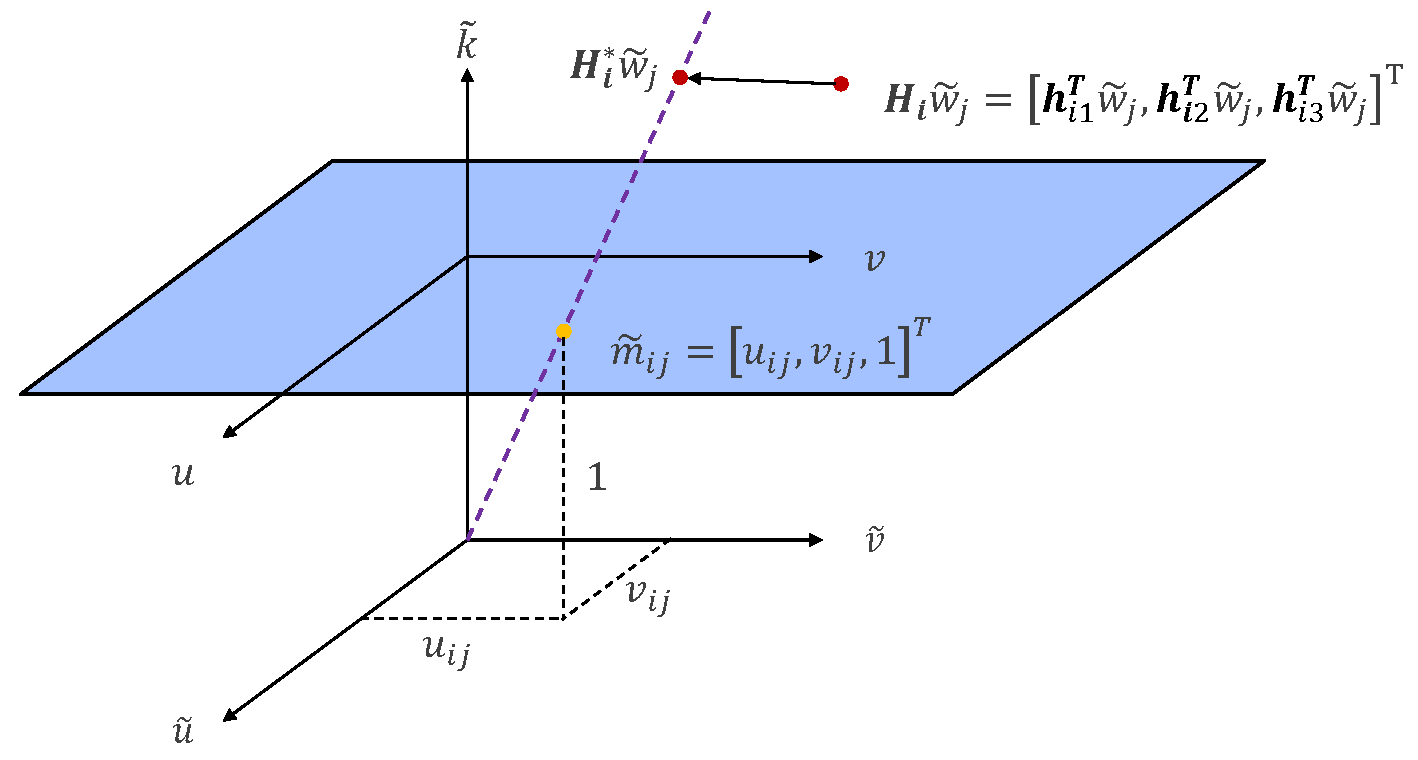
\includegraphics[width=0.7\linewidth]{./img/_zhang_corner_homography.pdf}
                \end{center}

                It can be shown that two vectors have the same direction if their cross product is $\nullvec$:
                \begin{align*}
                    \tilde{\vec{m}}_{i,j} \equiv \matr{H}_i \tilde{\vec{w}}_j 
                    &\iff
                        \tilde{\vec{m}}_{i,j} \times \matr{H}_i \tilde{\vec{w}}_j = \nullvec \iff
                        \begin{bmatrix} u_{i, j} \\ v_{i, j} \\ 1 \end{bmatrix} \times
                        \begin{bmatrix}
                            \vec{h}_{i, 1}^T \tilde{\vec{w}}_j \\ 
                            \vec{h}_{i, 2}^T \tilde{\vec{w}}_j \\ 
                            \vec{h}_{i, 3}^T \tilde{\vec{w}}_j
                        \end{bmatrix} =
                        \begin{bmatrix} 0 \\ 0 \\ 0 \end{bmatrix} 
                    \\
                    &\iff
                        \begin{bmatrix}
                            v_{i,j} \vec{h}_{i,3}^T \tilde{\vec{w}}_j - \vec{h}_{i, 2}^T \tilde{\vec{w}}_j \\
                            \vec{h}_{i, 1}^T \tilde{\vec{w}}_j - u_{i, j} \vec{h}_{i, 3}^T \tilde{\vec{w}}_j \\
                            u_{i, j} \vec{h}_{i, 2}^T \tilde{\vec{w}}_j - v_{i, j} \vec{h}_{i, 1}^T \tilde{\vec{w}}_j
                        \end{bmatrix} =
                        \begin{bmatrix} 0 \\ 0 \\ 0 \end{bmatrix} 
                    \\
                    &\iff
                        \underset{\mathbb{R}^{3 \times 9}}{\begin{bmatrix}
                            \nullvec_{1 \times 3} & -\tilde{\vec{w}}_j^T & v_{i,j} \tilde{\vec{w}}_j^T \\
                            \tilde{\vec{w}}_j^T & \nullvec_{1\times 3} & -u_{i,j} \tilde{\vec{w}}_j^T \\
                            -v_{i,j} \tilde{\vec{w}}_j^T & u_{i,j} \tilde{\vec{w}}_j^T & \nullvec_{1\times 3}
                        \end{bmatrix}}
                        \underset{\mathbb{R}^{9 \times 1}}{\begin{bmatrix}
                            \vec{h}_{i,1} \\ \vec{h}_{i,2} \\ \vec{h}_{i,3}
                        \end{bmatrix}}
                        =
                        \begin{bmatrix} 0 \\ 0 \\ 0 \end{bmatrix} 
                    & \text{\parbox[t]{5cm}{$\vec{h}_{*}^T \tilde{\vec{w}}_j = \tilde{\vec{w}}_j^T \vec{h}_{*}$\\and factorization}} \\
                    &\iff
                        \underset{\mathbb{R}^{2 \times 9}}{\begin{bmatrix}
                            \nullvec_{1 \times 3} & -\tilde{\vec{w}}_j^T & v_{i,j} \tilde{\vec{w}}_j^T \\
                            \tilde{\vec{w}}_j^T & \nullvec_{1\times 3} & -u_{i,j} \tilde{\vec{w}}_j^T \\
                        \end{bmatrix}}
                        \underset{\mathbb{R}^{9 \times 1}}{\begin{bmatrix}
                            \vec{h}_{i,1} \\ \vec{h}_{i,2} \\ \vec{h}_{i,3}
                        \end{bmatrix}}
                        =
                        \begin{bmatrix} 0 \\ 0 \end{bmatrix} 
                    & \text{\parbox{5cm}{only the first two\\equations are\\linearly independent}} \\
                \end{align*}
        \end{description}

        Given $c$ corners, a homogeneous overdetermined linear system of $2c$ equations to estimate the (vectorized) homography $\vec{h}_i$ is defined as follows:
        \[
            \underset{\mathbb{R}^{2c \times 9}}{
                \begin{bmatrix}
                    \nullvec_{1 \times 3} & -\tilde{\vec{w}}_1^T & v_{i,1} \tilde{\vec{w}}_1^T \\
                    \tilde{\vec{w}}_1^T & \nullvec_{1 \times 3} & -u_{i,1} \tilde{\vec{w}}_1^T \\
                    \vdots & \vdots & \vdots \\
                    \nullvec_{1 \times 3} & -\tilde{\vec{w}}_c^T & v_{i,c} \tilde{\vec{w}}_c^T \\
                    \tilde{\vec{w}}_c^T & \nullvec_{1 \times 3} & -u_{i,c} \tilde{\vec{w}}_c^T \\
                \end{bmatrix}
            }
            \underset{\mathbb{R}^{9 \times 1}}{
                \begin{bmatrix}
                    \vec{h}_{i, 1} \\ \vec{h}_{i, 2} \\ \vec{h}_{i, 3}
                \end{bmatrix}
            }
            =
            \nullvec_{2c \times 1}
            \Rightarrow
            \matr{L}_i \vec{h}_i = \nullvec
        \]
        With the constraint $\Vert \vec{h}_i \Vert = 1$ to avoid the trivial solution $\vec{h}_i = \nullvec$.

        The solution $\vec{h}_i^*$ is found by minimizing the norm of $\matr{L}_i \vec{h}_i$:
        \[
            \vec{h}_i^* = \arg\min_{\vec{h_i} \in \mathbb{R}^{9}} \Vert \matr{L}_i \vec{h}_i \Vert \text{ subject to } \Vert \vec{h}_i \Vert = 1
        \]
        $\vec{h}_i^*$ can be found using the singular value decomposition of $\matr{L}_i = \matr{U}_i \matr{D}_i \matr{V}_i^T$.
        It can be shown that $\vec{h}_i^* = \vec{v}_9$ where $\vec{v}_9$ is the last column of $\matr{V}_i$, associated with the smallest singular value.

        \begin{remark}
            This step minimizes an algebraic error.
        \end{remark}

    \item[Homographies non-linear refinement]
        The homographies $\matr{H}_i$ estimated at the previous step are obtained using a linear method and need to be refined as, for each image $i$, 
        the IRF coordinates $\matr{H}_i\vec{w}_j = \left( \frac{h_{i, 1}^T \tilde{\vec{w}}_j}{h_{i, 3}^T \tilde{\vec{w}}_j}, \frac{h_{i, 2}^T \tilde{\vec{w}}_j}{h_{i, 3}^T \tilde{\vec{w}}_j} \right)$
        of the world point $\vec{w}_j$ are still not matching the known IRF coordinates $\vec{m}_{i,j}$ of the $j$-th corner in the $i$-th image.
        \begin{figure}[H]
            \centering
            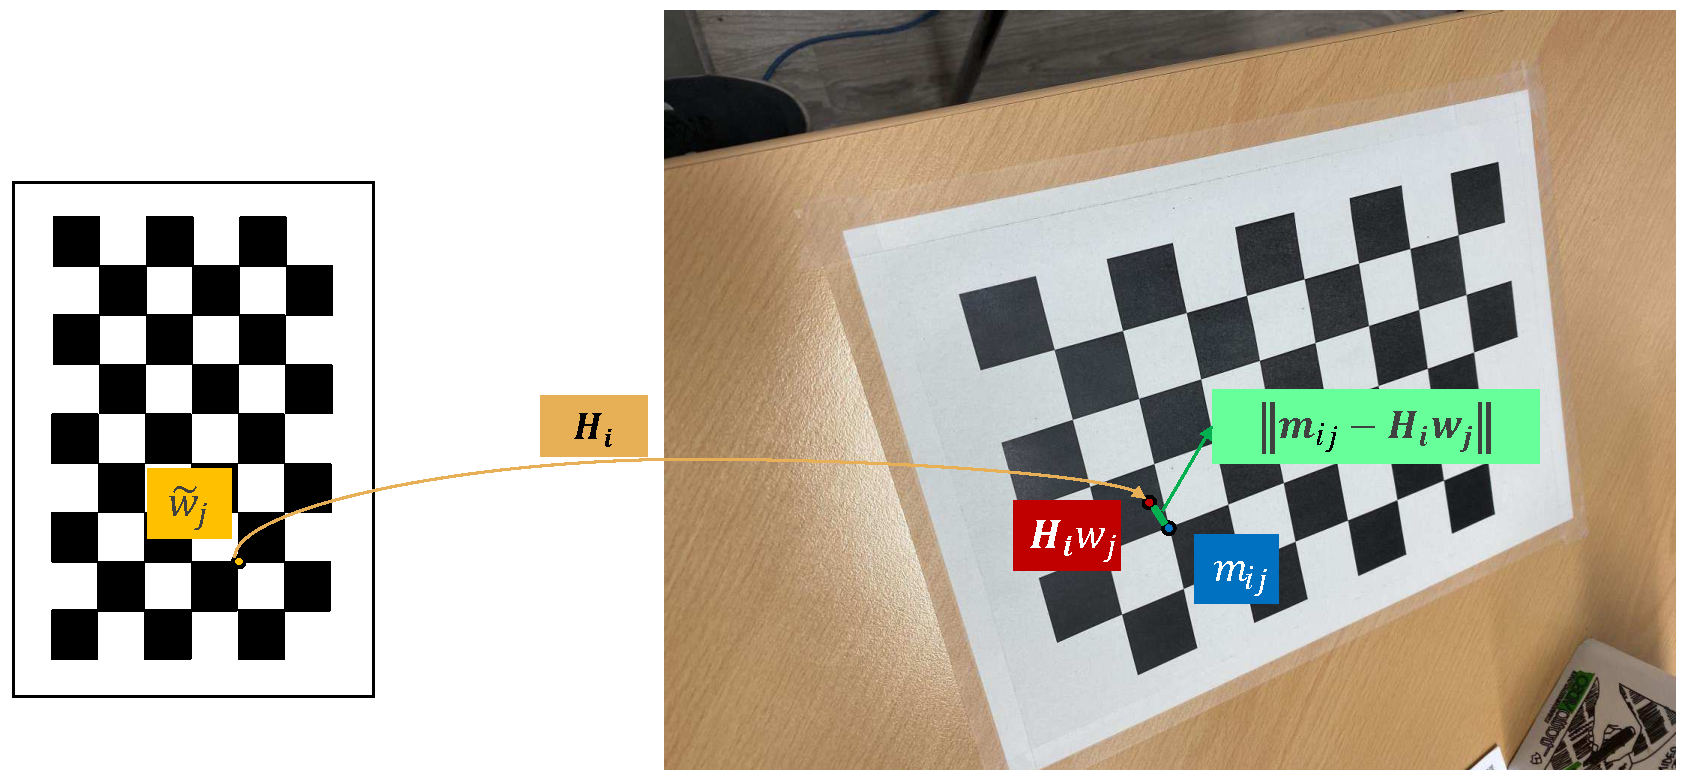
\includegraphics[width=0.7\linewidth]{./img/_homography_refinement.pdf}
        \end{figure}

        Given an initial guess for the homography $\matr{H}_i$, we can refine it through a non-linear minimization problem:
        \[ \matr{H}_i^* = \arg\min_{\matr{H}_i} \sum_{j=1}^{c} \Vert \vec{m}_{i,j} - \matr{H}_i \vec{w}_j \Vert^2 \]

        This can be solved using an iterative algorithm (e.g. Levenberg-Marquardt algorithm).

        \begin{remark}
            This step minimizes a geometric error.
        \end{remark}

    \item[Initial intrinsic parameters guess]
        From the PPM, the following relationship between intrinsic and extrinsic parameters can be established:
        \[
            \begin{aligned}
                \matr{P}_i &\equiv \matr{A}[\matr{R}_i | \vec{t}_i] = \matr{A} \begin{bmatrix} \vec{r}_{i,1} & \vec{r}_{i,2} & \vec{r}_{i,3} & \vec{t}_{i} \end{bmatrix} \\
                    &\Rightarrow \matr{H}_i = \begin{bmatrix} \vec{h}_{i,1} & \vec{h}_{i,2} & \vec{h}_{i,3} \end{bmatrix} = 
                        \begin{bmatrix} k\matr{A}\vec{r}_{i,1} & k\matr{A}\vec{r}_{i,2} & k\matr{A}\vec{t}_{i} \end{bmatrix}
                        & \text{By definition of $\matr{H}_i$} \\
                    &\Rightarrow (k\vec{r}_{i,1} = \matr{A}^{-1} \vec{h}_{i,1}) \land (k\vec{r}_{i,2} = \matr{A}^{-1}\vec{h}_{i,2})
            \end{aligned}
        \]
        Moreover, as $\matr{R}_i$ is an orthogonal matrix, the following two constraints must hold:
        \[
            \begin{split}
                \langle \vec{r}_{i,1}, \vec{r}_{i,2} \rangle = \nullvec &\Rightarrow 
                    \langle \matr{A}^{-1} \vec{h}_{i,1}, \matr{A}^{-1} \vec{h}_{i,2} \rangle = \nullvec \\
                    &\Rightarrow \vec{h}_{i,1}^T (\matr{A}^{-1})^T \matr{A}^{-1} \vec{h}_{i,2} = \nullvec
            \end{split}
        \]
        \[
            \begin{split}
                \langle \vec{r}_{i,1}, \vec{r}_{i,1} \rangle = \langle \vec{r}_{i,2}, \vec{r}_{i,2} \rangle &\Rightarrow
                    \langle \matr{A}^{-1} \vec{h}_{i,1}, \matr{A}^{-1} \vec{h}_{i,1} \rangle = \langle \matr{A}^{-1} \vec{h}_{i,2}, \matr{A}^{-1} \vec{h}_{i,2} \rangle \\
                    &\Rightarrow \vec{h}_{i,1}^T (\matr{A}^{-1})^T \matr{A}^{-1} \vec{h}_{i,1} = \vec{h}_{i,2}^T (\matr{A}^{-1})^T \matr{A}^{-1} \vec{h}_{i,2}
            \end{split}
        \]
        where $\langle \cdot, \cdot \rangle$ is the dot product.
        
        If at least 3 images have been collected, by stacking the two constraints for each image,
        we obtain a homogeneous system of equations that can be solved with SVD over the unknown $(\matr{A}^{-1})^T \matr{A}^{-1}$.

        Note that $(\matr{A}^{-1})^T \matr{A}^{-1}$ is symmetric, therefore reducing the number of independent parameters to 5 (6 with skew).

        Once $(\matr{A}^{-1})^T \matr{A}^{-1}$ has been estimated, the actual values of $\matr{A}$ can be found by solving a 
        traditional system of equations using the structure and results in $(\matr{A}^{-1})^T \matr{A}^{-1}$.

        \begin{remark}
            This step minimizes an algebraic error.
        \end{remark}

    \item[Initial extrinsic parameters guess]
        For each image, given the estimated intrinsic matrix $\matr{A}$ and the homography $\matr{H}_i$,
        it holds that:
        \[
            \begin{split}
                \matr{H}_i &= \begin{bmatrix} \vec{h}_{i,1} & \vec{h}_{i,2} & \vec{h}_{i,3} \end{bmatrix} =
                    \begin{bmatrix} k\matr{A}\vec{r}_{i,1} & k\matr{A}\vec{r}_{i,2} & k\matr{A}\vec{t}_{i} \end{bmatrix} \\
                    &\Rightarrow \vec{r}_{i,1} = \frac{\matr{A}^{-1} \vec{h}_{i,1}}{k} 
            \end{split}  
        \]
        Then, as $\vec{r}_{i,1}$ is a unit vector, it must be that $k = \Vert \matr{A}^{-1} \vec{h}_{i,1} \Vert$.

        Now, with $k$ estimated, $\vec{r}_{i,2}$ and $\vec{t}_{i}$ can be computed:
        \[ \vec{r}_{i,2} = \frac{\matr{A}^{-1}\vec{h}_{i,2}}{k} \hspace{3em} \vec{t}_{i} = \frac{\matr{A}^{-1}\vec{h}_{i,3}}{k} \]

        Finally, $\vec{r}_{i,3}$ can be computed as:
        \[ \vec{r}_{i,3} = \vec{r}_{i,1} \times \vec{r}_{i,2} \]
        where $\times$ is the cross-product. It holds that:
        \begin{itemize}
            \item $\vec{r}_{i,3}$ is orthogonal to $\vec{r}_{i,1}$ and $\vec{r}_{i,2}$.
            \item $\Vert \vec{r}_{i,3} \Vert = 1$ as the cross-product computes the area of the square defined by $\vec{r}_{i,1}$ and $\vec{r}_{i,2}$ (both unit vectors).
        \end{itemize}

        Note that the resulting rotation matrix $\matr{R}_i$ is not exactly orthogonal as:
        \begin{itemize}
            \item $\vec{r}_{i,1}$ and $\vec{r}_{i,2}$ are not necessarily orthogonal.
            \item $\vec{r}_{i,2}$ does not necessarily have unit length as $k$ was computed considering $\vec{r}_{i,1}$.
        \end{itemize}
        SVD for $\matr{R}_i$ can be used to find the closest orthogonal matrix by substituting the singular value matrix $\matr{D}$ with the identity $\matr{I}$.

        \begin{remark}
            This step minimizes an algebraic error.
        \end{remark}

    \item[Initial distortion parameters guess]
        The current estimate of the homographies $\matr{H}_i$ project WRF points into ideal (undistorted) IRF coordinates $\vec{m}_\text{undist}$ (this is an assumption).
        On the other hand, the coordinates $\vec{m}$ of the corners in the actual image are distorted.

        The original algorithm estimates the parameters of the radial distortion function defined as:
        \[
            \begin{bmatrix} x \\ y \end{bmatrix} = L(r) \begin{bmatrix} x_\text{undist} \\ y_\text{undist} \end{bmatrix} =
                (1 + k_1r^2 + k_2r^4) \begin{bmatrix} x_\text{undist} \\ y_\text{undist} \end{bmatrix}
        \]
        where $k_1$ and $k_2$ are parameters.

        \begin{remark}
            OpenCV uses a different method to estimate:
            \begin{itemize}
                \item 3 parameters $k_1$, $k_2$, $k_3$ for radial distortion.
                \item 2 parameters $p_1$, $p_2$ for tangential distortion.
            \end{itemize}
        \end{remark}

        Using the estimated intrinsic matrix $\matr{A}$, it is possible to obtain the CRF coordinates $(x, y)$ from the IRF coordinates $(u, v)$ 
        of $\vec{m}$ or $\vec{m}_\text{undist}$:
        \[
            \begin{bmatrix} ku \\ kv \\ k \end{bmatrix} \equiv \matr{A} \begin{bmatrix} x \\ y \\ 1 \end{bmatrix} \,\,\Rightarrow\,\,
            \begin{bmatrix} ku \\ kv \\ k \end{bmatrix} \equiv \begin{bmatrix} f_u x + u_0 \\ f_v y + v_0 \\ 1 \end{bmatrix} \,\,\Rightarrow\,\,
            \begin{bmatrix} x \\ y \end{bmatrix} = \begin{bmatrix} \frac{u-u_0}{f_u} \\ \frac{v-v_0}{f_v} \end{bmatrix}
        \]
        Then, the distortion equation can be rewritten in IRF coordinates as:
        \[
            \begin{split}
                \begin{bmatrix} \frac{u-u_0}{f_u} \\ \frac{v-v_0}{f_v} \end{bmatrix} &=
                    (1 + k_1r^2 + k_2r^4) \begin{bmatrix} \frac{u_\text{undist}-u_0}{f_u} \\ \frac{v_\text{undist}-v_0}{f_v} \end{bmatrix} \\
                &\Rightarrow \begin{bmatrix} u-u_0 \\ v-v_0 \end{bmatrix} = (1 + k_1r^2 + k_2r^4) \begin{bmatrix} u_\text{undist}-u_0 \\ v_\text{undist}-v_0 \end{bmatrix} \\
                &\Rightarrow \begin{bmatrix} u-u_0 \\ v-v_0 \end{bmatrix} - \begin{bmatrix} u_\text{undist}-u_0 \\ v_\text{undist}-v_0 \end{bmatrix} = 
                    (k_1r^2 + k_2r^4) \begin{bmatrix} u_\text{undist}-u_0 \\ v_\text{undist}-v_0 \end{bmatrix} \\
                &\Rightarrow \begin{bmatrix} u-u_\text{undist} \\ v-v_\text{undist} \end{bmatrix} = 
                    \begin{bmatrix}
                        (u_\text{undist} - u_0)r^2 & (u_\text{undist} - u_0)r^4 \\
                        (v_\text{undist} - v_0)r^2 & (v_\text{undist} - v_0)r^4
                    \end{bmatrix}
                    \begin{bmatrix} k_1 \\ k_2 \end{bmatrix}
            \end{split}
        \]
        With $n$ images with $c$ corners each, we obtain $2nc$ equations 
        to form a system $\vec{d} = \matr{D} \vec{k}$ in 2 unknowns $\vec{k} = \begin{bmatrix} k_1 & k_2\end{bmatrix}^T$.
        This can be solved in a least squares approach as:
        \[ \vec{k}^*  = \min_k \Vert \matr{D}\vec{k} - \vec{d} \Vert_2 = \matr{D}^\dagger \vec{d} = (\matr{D}^T\matr{D})^{-1} \matr{D}^T \vec{d} \]
        where $\matr{D}^\dagger$ is the pseudo-inverse of $\matr{D}$.

        \begin{remark}
            This step minimizes an algebraic error.
        \end{remark}

    \item[Parameters non-linear refinement]
        A final non-linear refinement of all the estimated parameters is done to obtain a solution closer to their physical meaning.

        Assuming i.i.d. noise, this is done through the maximum likelihood estimate (MLE) using the estimated parameters as starting point:
        \[ 
            \matr{A}^*, \vec{k}^*, \matr{R}_i^*, \vec{t}_i^* = 
                \arg\min_{\matr{A}, \vec{k}, \matr{R}_i, \vec{t}_i} \sum_{i=1}^n \sum_{j=1}^c 
                    \Vert \tilde{\vec{m}}_{i,j} - \hat{\vec{m}}(\matr{A}, \vec{k}, \matr{R}_i, \vec{t}_i, \tilde{\vec{w}}_j) \Vert^2
        \]
        where $\tilde{\vec{m}}_{i,j}$ are the known IRF coordinates in projective space of the $j$-th corner in the $i$-th image and
        $\hat{\vec{m}}(\cdot)$ is the projection from WRF to IRF coordinates using the estimated parameters.

        This can be solved using iterative algorithms.

        \begin{remark}
            This step minimizes a geometric error.
        \end{remark}
\end{description}



\section{Warping}

\begin{description}
    \item[Warp] \marginnote{Warp}
        Transformation of an image on the spatial domain.

        Given an image $I$, warping can be seen as a function $w$ that computes the new coordinates of each pixel:
        \[ u' = w_u(u, v) \hspace{2em} v' = w_v(u, v) \]

        The transformation can be:
        \begin{descriptionlist}
            \item[Rotation] 
                $\begin{bmatrix} u' \\ v' \end{bmatrix} = \begin{bmatrix} \cos\theta & -\sin\theta \\ \sin\theta & \cos\theta \end{bmatrix}\begin{bmatrix} u \\ v \end{bmatrix}$
            \item[Full homography]
                $k\begin{bmatrix} u' \\ v' \\ 1 \end{bmatrix} = 
                    \begin{bmatrix} h_{1,1} & h_{1,2} & h_{1,3} \\ h_{2,1} & h_{2,2} & h_{2,3} \\ h_{3,1} & h_{3,2} & h_{3,3} \end{bmatrix}\begin{bmatrix} u \\ v \\ 1 \end{bmatrix}$

        \end{descriptionlist}

        \begin{remark}
            Differently from warping, filtering transforms the pixel intensities of an image.
        \end{remark}
\end{description}


\subsection{Forward mapping}
\marginnote{Forward mapping}

Starting from the input image coordinates, apply the warping function to obtain the output image.

Output coordinates might be continuous and need to be discretized (e.g. truncated or rounded).
This might give rise to two problems:
\begin{descriptionlist}
    \item[Fold] More than one input pixel ends up in the same output pixel.
    \item[Hole] An output pixel does not have a corresponding input pixel.
\end{descriptionlist}

\begin{figure}[H]
    \centering
    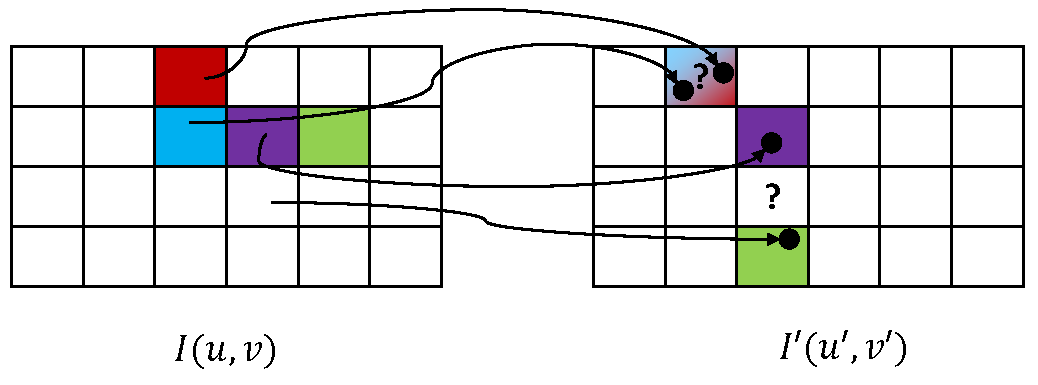
\includegraphics[width=0.55\linewidth]{./img/_forward_warping.pdf}
    \caption{Example of fold and hole}
\end{figure}


\subsection{Backward mapping}
\marginnote{Backward mapping}

Starting from the output image coordinates, use the inverse of the warping function $w^{-1}$ to find its corresponding input coordinates.
\[ u = w_u^{-1}(u', v') \hspace{2em} v = w_v^{-1}(u', v') \]

\begin{figure}[H]
    \centering
    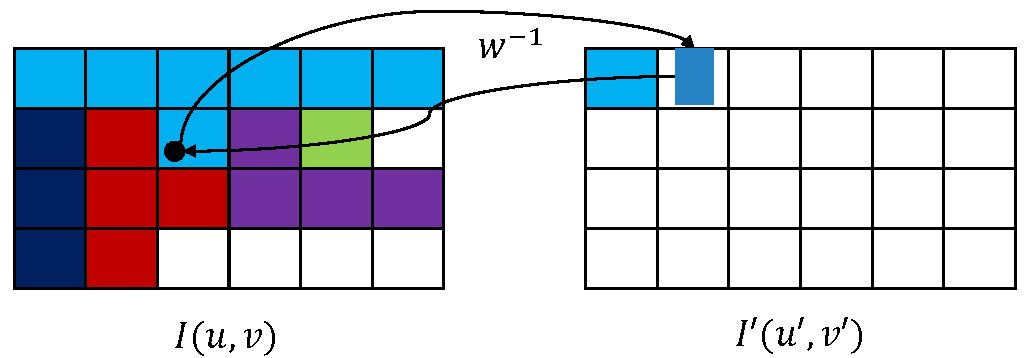
\includegraphics[width=0.55\linewidth]{./img/_backward_warping.pdf}
\end{figure}

The computed input coordinates might be continuous. Possible discretization strategies are:
\begin{itemize}
    \item Truncation.
    \item Nearest neighbor.
    \item Interpolation between the 4 closest pixels of the continuous point (e.g. bilinear, bicubic, \dots).
\end{itemize}


\begin{description}
    \item[Bilinear interpolation] \marginnote{Bilinear interpolation}
        Given a continuous coordinate $(u, v)$ and 
        its closest four pixels $(u_1, v_1), \dots, (u_4, v_4)$ with intensities denoted for simplicity as $I_i = I(u_i, v_i)$,
        bilinear interpolation works as follows:
        \begin{enumerate}
            \item Compute the offset of $(u,v)$ w.r.t. the top-left pixel:
                \[ \Delta u = u - u_1 \hspace{2em} \Delta v = v - v_1 \]
                \begin{figure}[H]
                    \centering
                    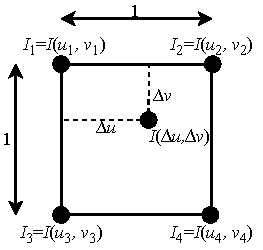
\includegraphics[width=0.25\linewidth]{./img/_warping_bilinear1.pdf}
                \end{figure}

            \item Interpolate a point $(u_a, v_a)$ between $(u_1, v_1)$ and $(u_2, v_2)$ in such a way that it is perpendicular to $(u,v)$.
                Do the same for a point $(u_b, v_b)$ between $(u_3, v_3)$ and $(u_4, v_4)$.
                The intensities of the new points are computed by interpolating the intensities of their extrema:
                \[ I_a = I_1 + (I_2 - I_1) \Delta u \hspace{2em} I_b = I_3 + (I_4 - I_3) \Delta u \]

                \begin{figure}[H]
                    \centering
                    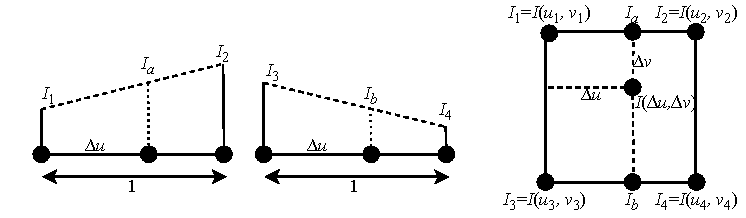
\includegraphics[width=0.7\linewidth]{./img/_warping_bilinear2.pdf}
                    \caption{In the figure, it is assumed that $I_1 < I_2$ and $I_3 > I_4$}
                \end{figure}
            
            \item The intensity $I(\Delta u, \Delta v) = I'(u', v')$ in the warped image is obtained by interpolating the intensities of $I_a$ and $I_b$:
                \[ 
                    \begin{split}
                        I'(u', v') &= I_a + (I_b - I_a) \Delta v \\
                        &= \Big( I_1 + (I_2 - I_1) \Delta u \Big) + \Big( \big( I_3 + (I_4 - I_3) \Delta u \big) - \big( I_1 + (I_2 - I_1) \Delta u \big) \Big) \Delta v \\
                        &= (1-\Delta u)(1 - \Delta v) I_1 + \Delta u (1-\Delta v) I_2 + (1-\Delta u) \Delta v I_3 + \Delta u \Delta v I_4
                    \end{split}
                \]
        \end{enumerate}

        \begin{remark}[Zoom]
            Zooming using nearest-neighbor produces sharper edges while bilinear interpolation results in smoother images.
            \begin{figure}[H]
                \centering
                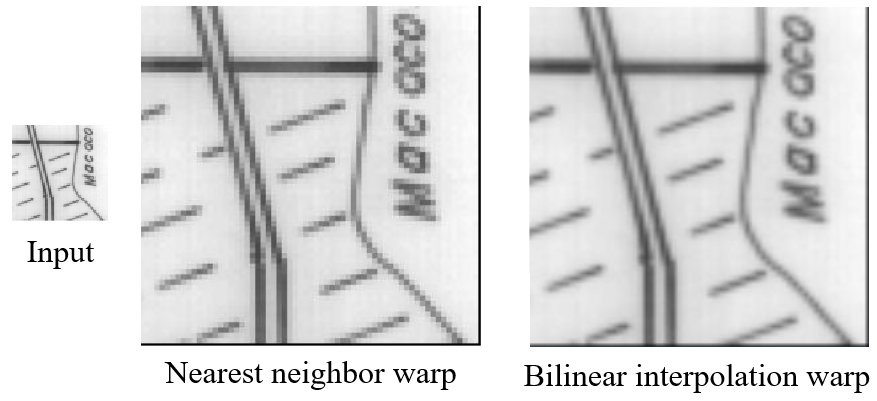
\includegraphics[width=0.5\linewidth]{./img/warp_zoom.png}
            \end{figure}
        \end{remark}

        \begin{remark}
            Nearest-neighbor is suited to preserve transition (e.g. zoom a binary mask while maintaining the 0s and 1s).
        \end{remark}
\end{description}


\subsection{Undistort warping}

Once a camera has been calibrated using Zhang's method, the lens distortion parameters can be used to obtain the undistorted image through backward warping.
\[
    \begin{split}
        w_u &= u_\text{undist} + (k_1 r^2 + k_2 r^4)(u_\text{undist} - u_0) \\
        w_v &= v_\text{undist} + (k_1 r^2 + k_2 r^4)(v_\text{undist} - v_0) \\
    \end{split}
\]
\[
    I'(u_\text{undist}, v_\text{undist}) = I\big( w^{-1}_u(u_\text{undist}, v_\text{undist}), w^{-1}_v(u_\text{undist}, v_\text{undist}) \big)
\]

Undistorted images enjoy some properties:
\begin{descriptionlist}
    \item[Planar warping] \marginnote{Planar warping}
        Any two images without lens distortion of a planar world scene ($z_W=0$) are related by a homography.
        \begin{figure}[H]
            \centering
            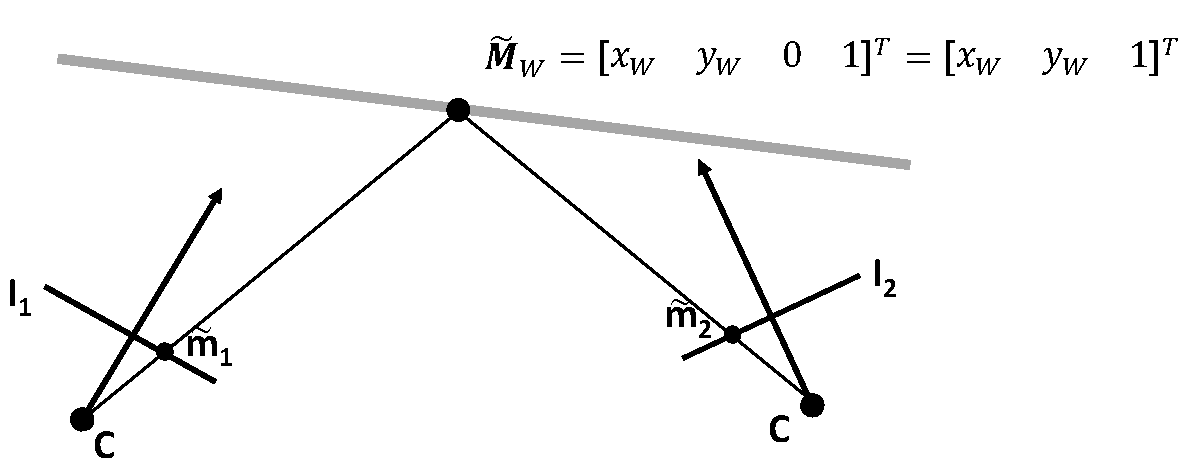
\includegraphics[width=0.5\linewidth]{./img/_warp_application1.pdf}
        \end{figure}
        Given two images containing the same world point, their image points (in projective space) are respectively given by a homography $\matr{H}_1$ and $\matr{H}_2$ 
        (note that with $z_w=0$, the PPM is a $3 \times 3$ matrix and therefore a homography):\\[-0.5em]
        \begin{minipage}{0.5\linewidth}            
            \[
                \begin{split}
                    \tilde{\vec{m}}_1 &= \matr{H}_1 \tilde{\vec{M}}_W \\
                    \tilde{\vec{m}}_1 &= \matr{H}_1 \matr{H}_2^{-1} \tilde{\vec{m}}_2 \\
                \end{split}
            \]
        \end{minipage}
        \begin{minipage}{0.5\linewidth}            
            \[
                \begin{split}
                    \tilde{\vec{m}}_2 &= \matr{H}_2 \tilde{\vec{M}}_W \\
                    \tilde{\vec{m}}_2 &= \matr{H}_2 \matr{H}_1^{-1} \tilde{\vec{m}}_1 \\
                \end{split}
            \]
        \end{minipage}\\[0.5em]
        Then, $\matr{H}_1 \matr{H}_2^{-1} = \matr{H}_{21} = \matr{H}_{12}^{-1}$ is the homography that relates $\tilde{\vec{m}}_2$ to $\tilde{\vec{m}}_1$
        and $\matr{H}_2 \matr{H}_1^{-1} = \matr{H}_{12} = \matr{H}_{21}^{-1}$ relates $\tilde{\vec{m}}_1$ to $\tilde{\vec{m}}_2$.

        \begin{remark}
            Only ground points on the planar section of the image can be correctly warped.
        \end{remark}

        \begin{example}[Inverse Perspective Mapping]
            In autonomous driving, it is usually useful to have a bird-eye view of the road.

            In a controlled environment, a calibrated camera can be mounted on a car to take a picture of the road in front of it.
            Then, a (virtual) image of the road viewed from above is generated.
            By finding the homography that relates the two images, it is possible to produce a bird-eye view of the road from the camera mounted on the vehicle.

            Note that the homography needs to be computed only once.

            \begin{figure}[H]
                \centering
                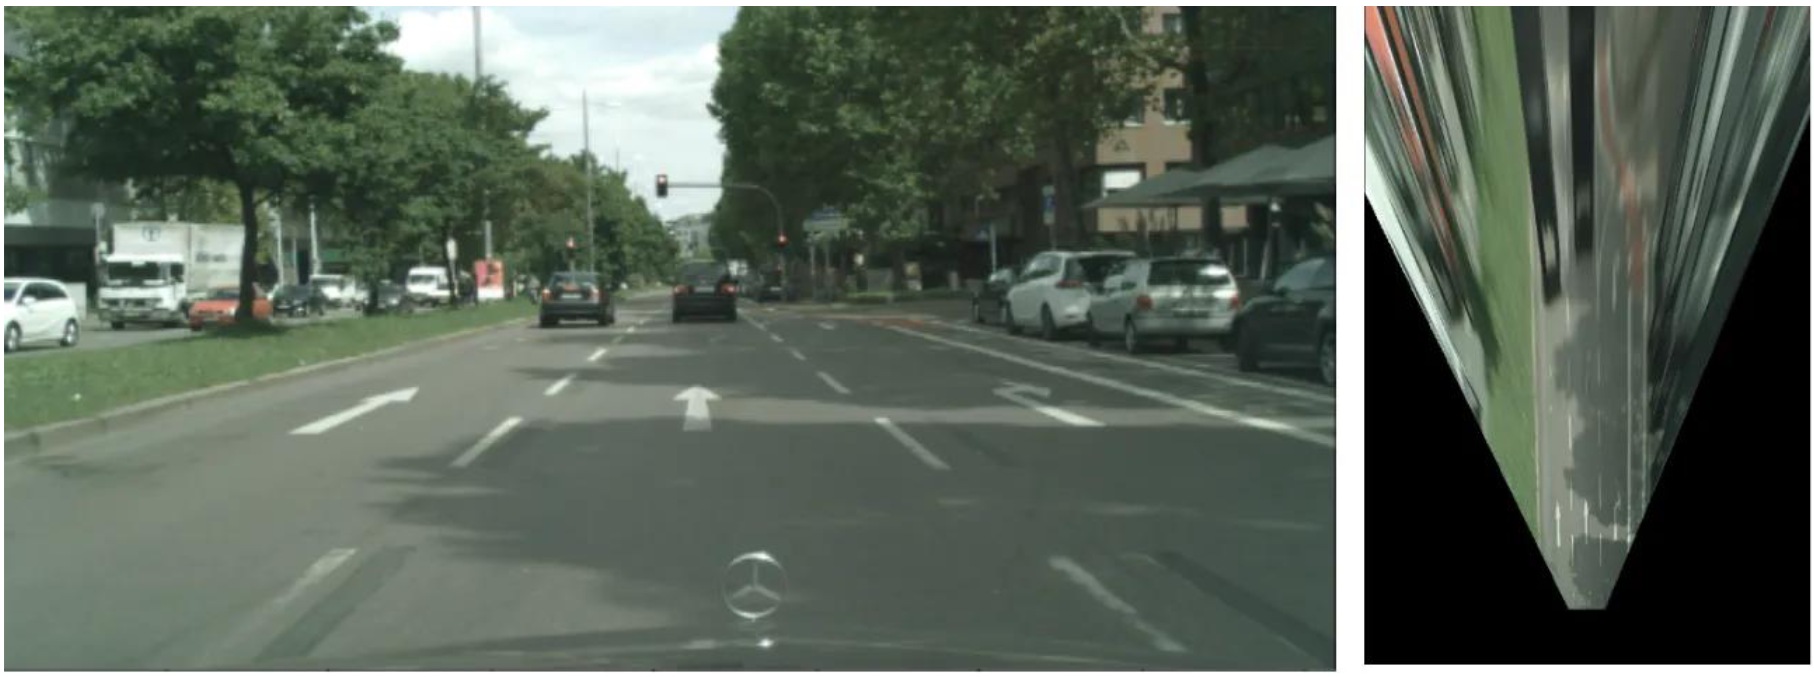
\includegraphics[width=0.7\linewidth]{./img/inverse_perspective_mapping.png}
            \end{figure}
        \end{example}

    \item[Rotation warping] \marginnote{Rotation warping}
        Any two images without lens distortion taken by rotating the camera about its optical center are related by a homography.
        \begin{figure}[H]
            \centering
            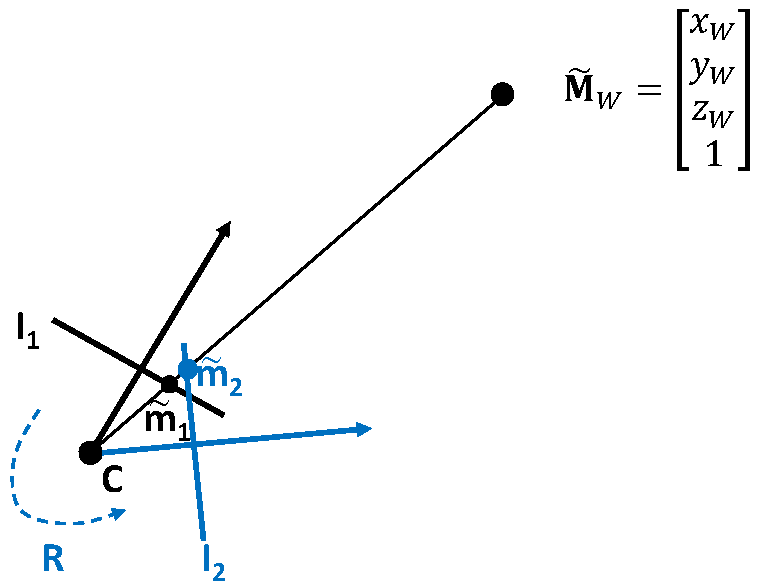
\includegraphics[width=0.35\linewidth]{./img/_warp_application2.pdf}
        \end{figure}
        It is assumed that the first image is taken in such a way that the WRF and CRF are the same (i.e. no extrinsic parameters).
        Then, a second image is taken by rotating the camera about its optical center.
        It holds that:\\[-0.5em]
        \begin{minipage}{0.5\linewidth}            
            \[
                \begin{split}
                    \tilde{\vec{m}}_1 &= \matr{A} [\matr{I} | \nullvec] \tilde{\vec{M}}_W = \matr{A}\tilde{\vec{M}}_W \\
                    \tilde{\vec{m}}_1 &= \matr{A}\matr{R}^{-1}\matr{A}^{-1} \tilde{\vec{m}}_2 \\
                \end{split}
            \]
        \end{minipage}
        \begin{minipage}{0.5\linewidth}            
            \[
                \begin{split}
                    \tilde{\vec{m}}_2 &= \matr{A} [\matr{R} | \nullvec] \tilde{\vec{M}}_W = \matr{A}\matr{R}\tilde{\vec{M}}_W \\
                    \tilde{\vec{m}}_2 &= \matr{A}\matr{R}\matr{A}^{-1} \tilde{\vec{m}}_1 \\
                \end{split}
            \]
        \end{minipage}\\[0.5em]
        Then, $\matr{A}\matr{R}^{-1}\matr{A}^{-1} = \matr{H}_{21} = \matr{H}_{12}^{-1}$ is the homography that relates $\tilde{\vec{m}}_2$ to $\tilde{\vec{m}}_1$
        and $\matr{A}\matr{R}\matr{A}^{-1} = \matr{H}_{12} = \matr{H}_{21}^{-1}$ relates $\tilde{\vec{m}}_1$ to $\tilde{\vec{m}}_2$.

        \begin{remark}
            Any point of the image can be correctly warped.
        \end{remark}

        \begin{example}[Compensate pitch or yaw]
            In autonomous driving, cameras should be ideally mounted with the optical axis parallel to the road plane and aligned with the direction of motion.
            It is usually very difficult to physically obtain perfect alignment 
            but a calibrated camera can help to compensate pitch (i.e. rotation around the $x$-axis)
            and yaw (i.e. rotation around the $y$-axis) by estimating the vanishing point of the lane lines.

            \begin{figure}[H]
                \centering
                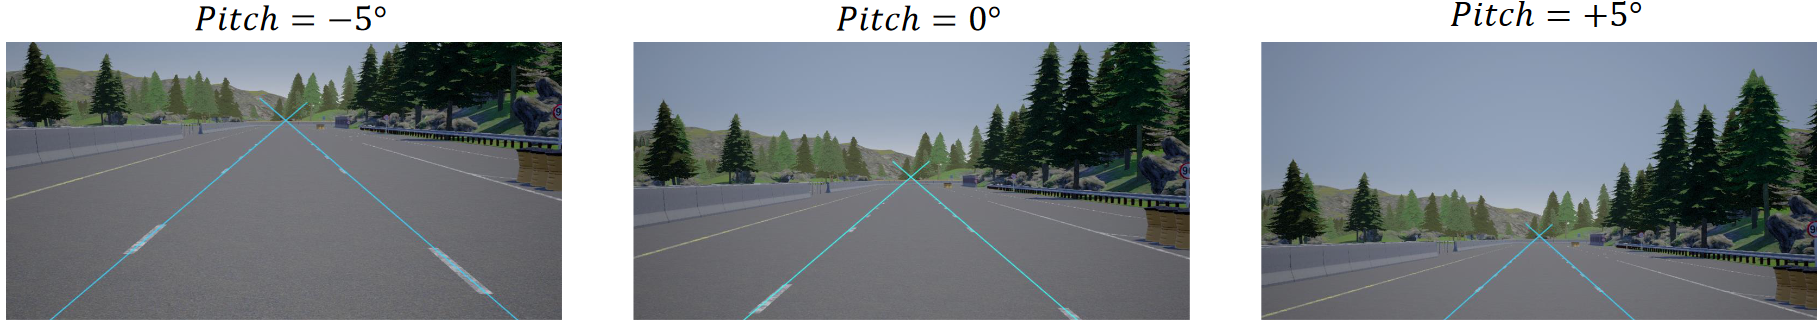
\includegraphics[width=0.85\linewidth]{./img/pitch_yaw_compensation.png}
            \end{figure}

            It is assumed that the vehicle is driving straight w.r.t. the lines and 
            that the WRF is attached to the vehicle in such a way that the $z$-axis is pointing in front of the vehicle.
            It holds that any line parallel to the $z$-axis has direction $\begin{bmatrix} 0 & 0 & 1 \end{bmatrix}^T$
            and their point at infinity in perspective space is at $\begin{bmatrix} 0 & 0 & 1 & 0 \end{bmatrix}^T$.

            The coordinates of the vanishing point are then obtained as:
            \[ 
                \vec{m}_\infty \equiv \matr{A}[\matr{R} | 0] \begin{bmatrix} 0 \\ 0 \\ 1 \\ 0 \end{bmatrix} 
                    \equiv \matr{A}\vec{r}_3 
                    \equiv \matr{A} \begin{bmatrix} 0 \\ \sin\beta \\ \cos\beta \end{bmatrix}
            \]
            where $\vec{r}_3$ is the third column of the rotation matrix $\matr{R}_\text{pitch} = \begin{bmatrix}
                1 & 0 & 0 \\ 0 & \cos\beta & \sin\beta \\ 0 & -\sin\beta & \cos\beta
            \end{bmatrix}$ that applies a rotation of $\beta$ degree around the $x$-axis.

            By computing the point at infinity, it is possible to estimate $\vec{r}_3 = \frac{\matr{A}^{-1} \vec{m}_\infty}{\Vert \matr{A}^{-1} \vec{m}_\infty \Vert_2}$
            (as $\vec{r}_3$ is a unit vector) and from it we can find the entire rotation matrix $\matr{R}_\text{pitch}$.

            Finally, the homography $\matr{A}\matr{R}_\text{pitch}\matr{A}^{-1}$ relates the pitched image to the ideal image.

            \indenttbox
            \begin{remark}
                The same procedure can be done for the yaw.
            \end{remark}
        \end{example}
\end{descriptionlist}